% g-2 Introduction
\chapter {Introduction} \label{ch:intro}

In particle physics, \gmtwo of the muon is an important and deep probe into \tsm (SM), because it can be both measured and calculated with very high precision.  The Fermilab \gmtwo experiment, E989, will measure the anomalous magnetic moment of the muon to an overall precision of \SI{140}{ppb}.  Parallel efforts in the particle physics theory community aim to calculate \mugmtwo to a comparable precision.

What is \gmtwo?  The quantity \gmtwo, well $(g\hbox{--}2)/2$, is the anomalous magnetic moment of a lepton,

\begin{equation}
\label{eqn:amm-lepton}
a_\ell = \left(\frac{g\hbox{--}2}{2}\right)_\ell.
\end{equation}

\noindent
The qualifier ``anomalous'' denotes a deviation from the value, $g \equiv 2$, in Dirac's theory of relativistic quantum mechanics.  The anomaly arises from off-shell interactions with particles in the quantum vacuum.  Such interactions are included in the modern theory of particle physics, which is based on quantum field theory.  The anomaly manifests as a small enhancement in the coupling of a leptons's spin vector to an external magnetic field.  The spin vector of a particle in a magnetic field precesses according to 

\begin{equation}
\label{eqn:omega-p}
\omega_{s} = g \frac{e B}{2 m}
\end{equation}

\noindent
where $g$ is the $g$-factor, $e$ is the magnitude of electron charge, $B$ is the magnetic field strength, and $m$ is the mass of the particle.  The $g$-factor is a particle-dependent constant that enters in the proportionality between the magnetic dipole moment, $\mu$, and the spin vector, $\vec{S}$:

\begin{equation}
\label{eqn:muon-mu}
\vec{\mu} = g \frac{e}{2 m} \vec{S}.
\end{equation}

The Fermilab \gmtwo experiment measures $a_\mu$ as the difference between two frequencies of muons in a magnetic storage field.  Inside of the dipole storage magnet, muon spin vectors precess in a manner consistent with equation \ref{eqn:omega-p} and muon momentum vectors rotate at the cyclotron frequency of the magnetic field as given by

\begin{equation}
\label{eqn:omega-c}
\omega_c = \frac{e B}{m_\mu}.
\end{equation}

\noindent
As muons circle around the storage magnet, the spin vector phase advances relative to the momentum vector at a rate exactly proportional to \gmtwo, a concept illustrated in figure \ref{fig:momentum-spin-vectors-ring}.  E989 measures the difference between the precession frequency and the cyclotron frequency, the anomalous spin precession frequency, $\omega_a$.  As stated above and shown in equation \ref{eqn:muon-g-2}, $\omega_a$ is directly proportional to the anomalous magnetic moment of the muon.

\begin{equation}
\label{eqn:muon-g-2}
\omega_a = \omega_s - \omega_c = \left( \frac{g_\mu - 2}{2} \right) \frac{e B}{m_\mu} = a_\mu \frac{e B}{m}
\end{equation}

\noindent
\textbf{Note:} the two labels, $a$ and \gmtwo, are used somewhat interchangeably to denote the anomaly.  Keep in mind that they technically differ by a factor of two.

\begin{figure}
\centering
\includegraphics[width=0.7\linewidth]{fig/momentum-spin-vectors-ring}
\caption{
    An illustration of the spin vector phase advance for muons trapped in a cyclotron.  The momentum vector undergoes perfect cyclotron motion and the spin vector edges forward due specifically to the anomalous magnetic moment.  The effect is exaggerated in the diagram. 
    \label{fig:momentum-spin-vectors-ring}
}
\end{figure}

% In order to properly introduce \gmtwo, it is instructive to touch upon some magnetic dipole moment fundamentals.  The next section presents motivational arguments for measuring muon \gmtwo. Then, a section details a brief overview of the experimental history of \mugmtwo, establishing context for current \mugmtwo experiments and highlighting the gradual rise of statistical tension between measured and calculated results.  And, finally, a section on the state of theory illuminates the types of contributions that affect \mugmtwo and which models may resolve the experimental results.

\section{Magnetic Dipole Moments}

\subsection{Definition}
Classically, an entity attains a magnetic moment, $\vec{\mu}$, when the object has a specific correlation between the motion of its electric charge and the physical space that it occupies.  Equation \ref{eqn:magnetic-moment-integral} illustrates how to calculate such a correlation for a body \cite{jackson}.  The analogous macro-scale quantity uses the term spin polarization or magnetization, $\vec{M}$, defined in equation \ref{eqn:polarization-sum}.

\begin{equation}
\label{eqn:magnetic-moment-integral}
\vec{\mu} = \frac{1}{2} \int \vec{r} \times \vec{j} \,dV
\end{equation}

\begin{equation}
\label{eqn:polarization-sum}
\vec{M} = \sum_i \vec{\mu}_i
\end{equation}

\noindent
Equation \ref{eqn:magnetic-moment-integral} can be re-framed in terms of angular momentum, $\vec{l}$, and charge density, $\rho$, by noting that $\vec{j} = \rho \, \vec{p}/m$ and $\vec{l} = \vec{r} \times \vec{p}$.

\begin{equation}
\label{eqn:magnetic-moment-integral-2}
\vec{\mu} = \frac{g}{2 m} \int \rho \, \vec{l} \,dV
\end{equation}

Equation \ref{eqn:magnetic-moment-integral-2} works for classical angular momentum and orbital angular momentum $\vec{L}$, however, in the case of intrinsic spin angular momentum, $\vec{S}$, there is a caveat.  A proportionality constant, the $g$-factor, must be included in the spin calculation of the equation giving rise to equation \ref{eqn:spin-mu} for particle magnetic moments that arise due to spin.

\begin{equation}
\label{eqn:spin-mu}
\vec{\mu} = g \frac{e}{2 m}\vec{S}
\end{equation}

\noindent
The $g$-factor, $g$, represents the coupling strength of a particle to the type of interactions mediated by magnetic fields.  This quantity can vary extensively between different particles for instance, the proton $g$-factor is 5.5 \cite{codata}, and the neutron has a $g$-factor of -3.8 \cite{codata}.  It is worth noting that naively the neutron should not even have a magnetic moment due to a lack of net charge.  For a point-like particle, the $g$-factor predicted by Dirac Equation is exactly 2.  However, for charged leptons, the $g$-factor is slightly larger than 2, hence, the anomalous magnetic moment.

\subsection{Properties}

\subsubsection{Alignment with External Fields}
Intuitively, a magnetic moment is similar to a macroscopic magnet that nearly everyone is familiar with.  The most prominent behavior of magnets is a tendency to align with external magnetic fields.  Magnets align to minimize potential energy in the external field as given by equation \ref{eqn:spin-b-field-potential}. 

\begin{equation}
\label{eqn:spin-b-field-potential}
U = -\vec{\mu} \cdot \vec{B}
\end{equation}

\noindent 
Such behavior is exploited in compasses to align with the Earth's magnetic North Pole and seen with bar magnets where opposite ends attract.  Though the examples are macro-scale, this behavior persists statistically in the micro-scale as well.

\subsubsection{Spin Precession}
Precession is another important but lesser known behavior of magnets.  Precession actually arises from the same force which aligns a magnet in an external magnetic field.  A more familiar analogue comes from the spinning top example.  The child's toy receives a torque when the normal force on the top's tip and the ground is misaligned with the center of mass as illustrated in figure \ref{fig:spinning-top-precession}.

\begin{equation}
\label{eqn:top-torque-equation}
\vec{\tau} = \vec{r} \times \vec{F}_{N}
\end{equation}

\begin{figure}
\centering
\includegraphics[width=0.7\linewidth]{fig/spinning-top-precession}
\caption{
    The spinning top example of precession as a force diagram.  A torque arises from the off-center normal force, and that torque causes the top to precess at $\omega_p$.  The spinning top diagram was created by Xavier Snelgrove and found in the Wikipedia article for precession. 
    \label{fig:spinning-top-precession}
}
\end{figure}

\noindent
While the top is stabilized by rotational inertia, the induced torque causes the body to rotate about the top's tip.  The magnetic moment case is realized by allowing the normal force to be replaced by the Lorentz force from the external magnetic field on the effective currents in an object with a non-zero magnetic moment, equation \ref{eqn:mu-torque-equation}.

\begin{equation}
\label{eqn:mu-torque-equation}
\vec{\tau} = \vec{\mu} \times \vec{B}
\end{equation}

\noindent
The induced torque causes the magnetic moment vector to rotate in plane orthogonal as prescribed by equation \ref{eqn:larmor-precession}. The behavior is known as Larmor precession.

\begin{equation}
\label{eqn:larmor-precession}
\omega_L = \frac{\mu B}{2 m}
\end{equation}

\section{Muon Attributes} \label{sec:muon-attributes}

Muons are identical to electrons in most properties.  Both particles are charged leptons and lepton universality posits that they are identical except for mass and the fact that muons are intrinsically unstable.  Together with the tauon, they complete the charged lepton particle family.  For a bit more context, examine table \ref{tab:leptons} which enumerates lepton properties compiled by the Particle Data Group \cite{pdg-2016}.

\begin{table}[h]
\label{tab:leptons}
\caption{Lepton Properties}
\centering
\begin{tabular}{| l | c | c | c |}
    \hline
    Property & $e$ & $\mu$ & $\tau$ \\
    \hline
    charge   & -1   & -1   & -1  \\
    spin     & 1/2  & 1/2  & 1/2 \\
    mass     & \SI{0.511}{\MeV/c}   & \SI{105.7}{\MeV/c}   & \SI{1776.9}{\MeV/c} \\
    lifetime & \SI{>2.0e36}{\second} & \SI{2.2e-6}{\second} & \SI{290.3e-15}{\second} \\
    primary decay & None & $\mu \rightarrow e \, \bar{\nu}_e \, \nu_\mu$ & 
    $\tau \rightarrow \mu \, \bar{\nu}_\mu \, \nu_\tau$ \\
    \hline
\end{tabular}
\end{table}

\subsection{Decay Chain}

The pion decay chain is commonly used to produce muons.  The principle branch from pion decay produces muons with very high probability, more than \SI{99.9}{\percent} \cite{pdg-2016}.  Similarly, the muon decays into an electron and two neutrinos with nearly \SI{100}{\percent} probability \cite{pdg-2016}.  The decay formulas are shown in equation \ref{eqn:pion-decay-chain}.

\begin{equation}
\label{eqn:pion-decay-chain}
\begin{aligned}
\pi^+ & \rightarrow \mu^+ \bar{\nu}_\mu  \hspace{5em} & \pi^- & \rightarrow \mu^- \nu_\mu \\
\mu^+ & \rightarrow e^+ \bar{\nu_e} \nu_\mu  \hspace{5em} & \mu^- & \rightarrow e^- \nu_e \bar{\nu}_\mu\\
\end{aligned}
\end{equation}

\subsubsection{Pion Decay}

The two-body decay is isotropic in the pion rest frame and imparts \SI{59.4}{\GeV} of the pion rest energy to the (anti-)neutrino and \SI{75.6}{\GeV} to the muon.  In the SM, neutrinos are always produced with left-handed chirality meaning that the direction of the spin vector and the momentum vector are anti-aligned.  Conservation of angular momentum then forces the muon produced via pion decay to have the same chirality as the neutrino in the pion rest frame.  

The decay lends itself to production of spin polarized muons.  Here, polarization means alignment of the spin vector with the lab frame momentum vector rather than with the magnetic field as in the previous section.  When the isotropic decay is boosted into the lab frame for a pion beam, both the highest energy (forward decay) or lowest energy (backward decay) muons exhibit strong spin polarization.  As such momentum selection can be used to achieve a highly polarized muon beam. 

\begin{figure}
\centering
\includegraphics[height=5em]{fig/pion-decay-diagram}
\caption{
    A diagram depicting pion decay in the rest frame.  The spin vectors are shown in white and momentum vectors in color for the decay.  Both the muon and the neutrino receive half the rest mass of the pion.  The neutrino needs to have left-handed chirality, so both the neutrino and the muon are emitted with spin and momentum vectors anti-aligned.  For the $\pi^+$ decay, the particles are emitted with right-handed chirality.
    \label{fig:muon-decay-diagram}
}
\end{figure}

\subsubsection{Muon Decay}

The muon decay is a bit more complicated than pion decay, since the process is three-body instead of two-body.  A common framing for discussions of muon decay is the differential decay rate, $n(y)$, and asymmetry function, $a(y)$, over the range of possible muon energies, $y=E/E_{max}$ \cite{e989-tdr}.  The differential decay rate, also called the Michel Spectrum, is a proxy for the overall probability of a decay electron with the energy $y$.  The asymmetry function represents the likelihood of the decay electron momentum being in the direction of the muon spin.  Both functions are normalized to have a maximum value of one.  The decay functions for the muon rest frame in equation \ref{eqn:muon-decay-rest-frame}, and the corresponding plots are shown in figure \ref{fig:muon-decay-rest-frame}.

\begin{align}
\label{eqn:muon-decay-rest-frame}
n_{rest}(y) & = y^2(3 - 2 y) & a_{rest}(y) & = \frac{2 y - 1}{3 - 2y}
\end{align}

\begin{figure}
\centering
\includegraphics[width=0.7\linewidth]{fig/muon-decay-distributions-rest-frame}
\caption{
    The plot depicts characteristics of the muon decay in the rest frame.  The decay rate, $n(y)$, and the decay asymmetry, $a(y)$, are shown as a function of fractional energy, $y=E/E_{max}$.
    \label{fig:muon-decay-rest-frame}
}
\end{figure}

It is instructive to examine the extreme cases where both neutrinos are emitted in the same direction as shown in figure \ref{fig:muon-decay-diagram}, and the case where they have opposing momentum directions. 

\begin{figure}
\centering
\includegraphics[height=5em]{fig/muon-decay-diagram}
\caption{
    A diagram depicting the spin vectors in white and momentum vectors in color for muon decay. Together, the two neutrinos emitted in parallel carry away half the muon's rest mass in energy and no angular momentum.  The electron then receives the other half of the muon's rest mass energy, and momentum in the direction of the muon's spin. 
    \label{fig:muon-decay-diagram}
}
\end{figure}

The first case is the highest energy decay electron, the two neutrinos receive slight less than half the decay energy and the electron receives slightly more than half.  The neutrino/anti-neutrino pair carry away no angular momentum, because the neutrino must have left-handed chirality and the anti-neutrino must have right-handed chirality, opposing spins.  The decay electron then must carry the spin of the parent muon.

The second case is the lowest energy decay electron, the neutrino and the anti-neutrino each receive half the rest mass of the muon.  The electron is produced nearly at rest in this case.  The angular momentum carried by the neutrinos in this case is no longer zero, but rather one.  The electron then will be produced with spin in the opposite direction to the parent muon.

\section{Motivation for \mugmtwo}
There are two major questions that need answers to specifically motivate the muon \gmtwo experiment.  The first question is: ``Why measure the anomalous magnetic moment?'', and the second question is: ``Why use muons?''.

\subsubsection{Why \gmtwo?}
To the first question, there are many appropriate replies.  One answer is that it is a simple measurement in principle.  The experimenters need a spin polarized volume of leptons, an external magnetic field, and a technique to determine the spin direction. Another, more phenomenological answer is that contributions to \gmtwo come from the full gamut of fundamental interactions and constants of the universe in the SM: Quantum Electrodynamics (QED), Electro-Weak Interactions (EW), and Quantum Chromodynamics (QCD) all playing important roles. It traverses the entirety of Standard Model interactions aside from gravity. Precision measurements of \gmtwo are somewhat unique in this regard.  Couple that with the fact that \gmtwo is measurable and calculable to high precision, and it's no wonder that \gmtwo  has fascinated experimentalists and theorists for so many years.

\subsubsection{Why muons?}
And, to the second question, there are physics considerations and practical considerations.  The physics considerations weigh in with the desire for sensitivity to small effects predicted by the Standard Model.  A more precise measurement enhances the visibility of small effects much like a microscope enhances optically small characteristics.  The electron \gmtwo has already been measured with around 2,000 times more precision \cite{g-e-measurement}, so why not just measure $g_e$ even more precisely?  Well, simply put the physics contributions for $g_e$ and $g_\mu$ are just different.  Higher order interactions with particles of larger masses contribute with mass suppression terms, $\propto (\frac{m_\ell}{M})^2$, or possibly an even higher power!  These interactions mostly manifest in the EW and QCD sector.  The relative mass ratio between the electron and the muon enhances the sensitivity to these terms by a factor of $(\frac{105.66}{0.511})^2 \approx 43,000$ \cite{the-muon-g-2}!  Even though $g_e$ can be measured to much higher precision, $g_\mu$ is still around 2,000 times more sensitive to large mass contributions.  To that end, the electron \gmtwo is a deeper probe of QED and the muon \gmtwo is a more rounded probe of the SM.  

The preceding argument raises a further question though: ``Why not use the $\tau$?''.  The answer is really a practical consideration; the ephemeral $\tau$ has a lifetime of only \SI{0.29}{\femto\second} compared to \SI{2.2}{\micro\second} for the $\mu$ \cite{codata}.  The $\tau$ also has many decay modes rather than a single dominant one like the muon.  While the $\tau$ particle would be appealing if a significant enough Lorentz boost could be achieved and a clean method to understand the decay modes was presented, an experiment using $\tau$ particles is simply not practical with current technology.

\section{The History of Experiments} \label{sec:history-expt}

\subsection{Basic Principles}
What then, one might ask, are the bare necessities to perform the \gmtwo experiment?  Number one is a reliable source of spin polarized muons, the higher the net polarization the better.  Next, there must be a method to store the muons in an external magnetic field while they precess.  Recall that the experiment measures a frequency, so longer storage time increases the overall precision. Muon storage can be achieved through a cyclotron magnet as in older experiments or a magnetic storage ring as in many newer experiments.  The third necessity is a method by which to measure the direction of the muon spin vector over time.  Measuring the spin direction relies on the fact that spin information is transfered to the momentum of the decay electron.  The detector could be as simple as a forward/backward electron sensitive detector that measures decay electrons.  The last requirement is a method to characterize the magnetic field experienced by the muons as they precess.  Keep these points in mind as the historical experiments are discussed in the following sections.

\subsection{Anomaly Detection and Parity Violation}

The notion that $g \ne 2$ had to be reconciled with experiment as measurement precision progressed and statistical tensions arose with the values predicted by theory.  Deviations from a pure Dirac particle for leptons were first observed in hyperfine splitting measurements of several different isotopes by Kusch and Foley in 1947 \cite{kusch-foley}.  The theory community quickly resolved the discrepancy when Julian Schwinger released his seminal paper introducing corrections from quantum field fluctuations in 1948 \cite{schwinger}.  The paper describes a now standard QED calculation of the lowest order self-interaction term for leptons emitting and reabsorbing photons, see figure \ref{fig:schwinger-diagram}.  The Schwinger term brought experiment and theory back into good agreement, an early triumph of QED:

\begin{equation}
\label{eqn:schwinger-correction}
a_{_{Schwinger}} = \frac{\alpha_{_{QED}}}{2\pi}.
\end{equation}

\begin{figure}
\centering
\includegraphics[height=\fdh]{fig/schwinger-diagram}
\caption{The Feynman diagram for the so-called Schwinger term. The propagating lepton radiates a photon, interacts with the magnetic field via a disconnected photon and reabsorbs the radiated photon.  The contribution to $a_\mu$ from the interaction is $\frac{\alpha}{2\pi}$. \label{fig:schwinger-diagram}}
\end{figure}

The first detection of a magnetic moment anomaly from measurements of free electrons came later, and in muons much later.  The first measurement of $g_e$ was done in 1953 by H. R. Crane, et al. \cite{g-e-crane}.  Subsequent theoretical calculations and supporting experimental measurements established $g_e$ as the most precisely predicted and measured quantity in QED \cite{g-e-measurement}.  As for measuring $g_\mu$, it wasn't clear how to properly control the polarization of the muons, until parity violation of the weak interaction was understood \cite{lee-yang, wu-expt}.  With parity violation inherent in the weak interaction, researchers quickly realized that a pion beam would decay into muons polarized along the beam direction (see section \ref{sec:muon-attributes} for more detail on pion decay).

\subsection{CERN-I (1958-1962)}
Building off the weak parity revelation, researchers measured $g_\mu$ for the first time.  In 1960 Columbia personnel measured the quantity to $5\%$ uncertainty, and not long after in 1961 a more precise measurement was performed at CERN.  The experiment worked by injecting relatively low energy, \SI{83}{\MeV}, muons into a long, narrow magnetic trap where the polarized muons would undergo both cyclotron motion and lateral drift, see figure \ref{fig:cern-i-diagram}. At the opposite end of the magnet, the muons were ejected, tagged for storage time, and stopped where the momentum direction of the decay electron was recorded as either forward or backward.  Using this technique CERN scientists were able to achieve a precision of $0.4\%$ \cite{cern-i}.  At the achieved precision, a deviation of $1.6\,\sigma$ was present between the measured value and the value predicted by the Schwinger term \cite{47y-muon-g-2}.

\begin{equation}
\label{eqn:cern-i-results}
a_\mu = 116\,500\,000 (500\,000) \times 10^{-11}
\end{equation}

\begin{figure}
\centering
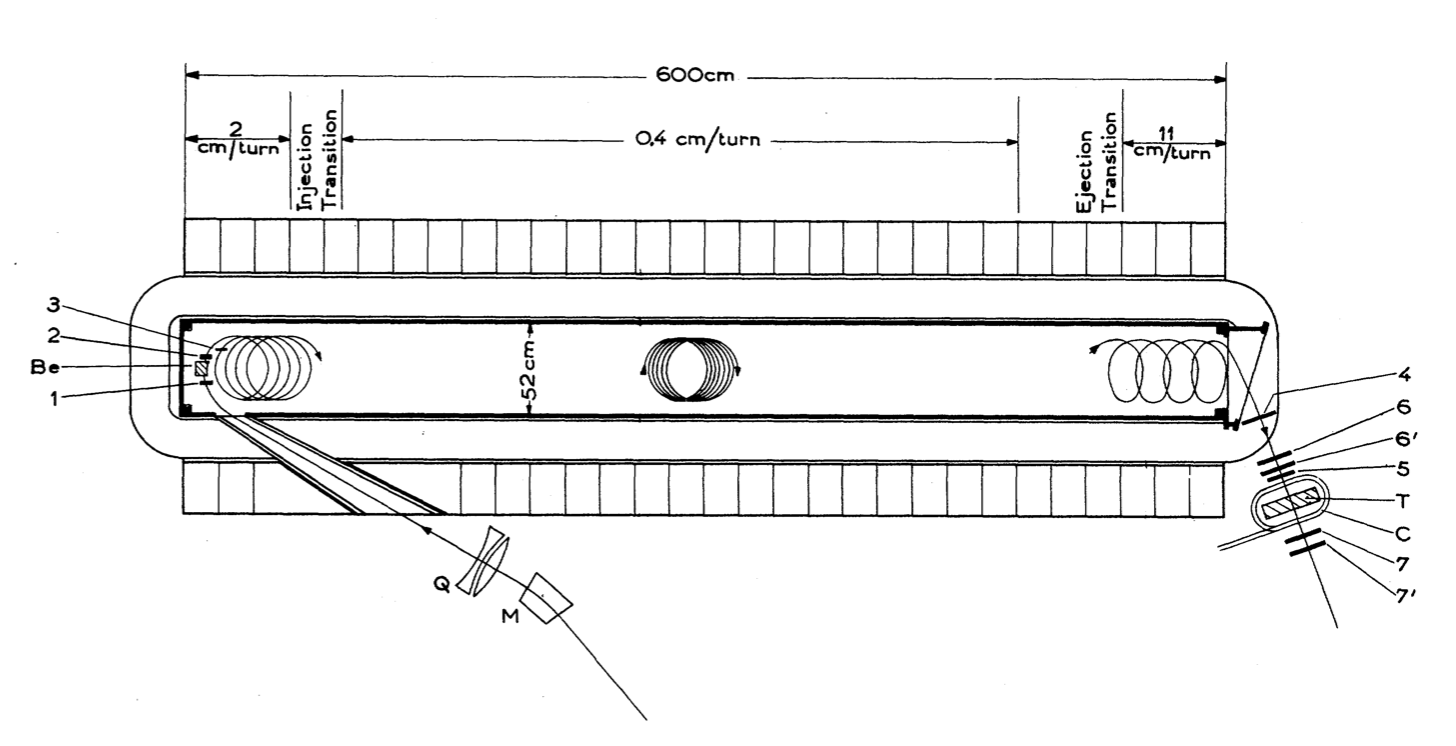
\includegraphics[width=0.9\linewidth]{fig/cern-i-diagram.png}
\caption{A diagram of the experimental setup in the first muon \gmtwo experiment at CERN from the original paper \cite{cern-i}. The muons enter from the lower left, go through the energy moderator to put the cyclotron radius at \SI{19}{\cm}, drift and circle toward the ejection side of the magnetic field, escape from the magnet, stop in the fiducial block, and decay into an electron with momentum correlated to the spin direction. \label{fig:cern-i-diagram}}
\end{figure}

\subsection{CERN-II (1962-1968)}
The second iteration of \mugmtwo at CERN improved by a factor of 15 over the first.  CERN-II was the first \mugmtwo experiment to use the now familiar magnetic storage ring as shown in figure \ref{fig:intro-cern-ii-storage-ring}.  The storage ring design allowed the experimenters to measure $a_\mu$ directly as opposed to $g_\mu$ as explained near the beginning of the chapter. In order to store muons, the experiment injected a beam of protons which hit a pion production target.  A slice of the pion production phase space matched the momentum acceptance of the ring well enough to remain for several revolutions. The stored muons were mostly forward decays that lost a bit of energy and matched the ring's momentum acceptance.  The decay electrons curled inward to produce signals in electron counting detectors at a rate that modulated at the $\omega_a$.  The injected muons had a relativistic $\gamma$ of 12 which allowed the researchers to increase the observation time of muon spin precession to more than 130 $\mu s$.  The increased duration led to improved determination of $a_\mu$ to \ppm{270} \cite{47y-muon-g-2}.

\begin{equation}
\label{eqn:cern-ii-results}
a_\mu = 116\,616\,000 (31\,000) \times 10^{-11}
\end{equation}

\begin{figure}
\centering
\includegraphics[width=0.7\linewidth]{fig/intro-cern-ii-storage-ring}
\caption{
    The first muon storage ring used in the CERN-II experiment.  Pions were injected and a fraction of the forward decay muons matched the ring's momentum acceptance.  Those polarized muons orbited the ring until decaying into electrons which activated the detectors.  The electron rate signal was used to extract $a_\mu$.
    \label{fig:intro-cern-ii-storage-ring}    
}
\end{figure}

\subsection{CERN-III (1969-1976)}
The third CERN muon \gmtwo experiment was also the last.  A major innovation introduced in CERN-III was use of the so-called ``magic'' momentum. Observe equation \ref{eqn:full-omega-a}, the expression for spin precession in electromagnetic fields for a relativistic muon.

\begin{equation}
\label{eqn:full-omega-a}
\vec{\omega}_a = \frac{e}{m} \left[ a_\mu \vec{B} - \\
\left(a_\mu - \frac{1}{\gamma^2 - 1} \right) \\
\frac{\vec{\beta} \times \vec{E}}{c} \right]
\end{equation}

\noindent A muon beam at a very specific momentum, \pmagic, cancels the effects of radial electric fields which allows electrostatic focusing to be used on the muon beam instead of magnetic gradient focusing.  The perturbations from magnetic focusing were a large source of uncertainty in the previous experiment.  Another major innovation for the third CERN experiment was the use of pion injection instead of proton injection.  The measurement techniques of CERN-III were similar to CERN-II.  The new magnetic storage ring constructed for the experiment is shown in figure \ref{fig:intro-cern-iii-storage-ring}.  With the achieved improvements, the CERN team was able to drive down the uncertainty on $a_\mu$ to \ppm{7} \cite{47y-muon-g-2}, nearly a 40-fold improvement!

\begin{equation}
\label{eqn:cern-iii-results}
a_\mu = 116\,592\,300 (800) \times 10^{-11}
\end{equation}

\begin{figure}
\centering
\includegraphics[width=0.7\linewidth]{fig/intro-cern-iii-storage-ring}
\caption{
    The second muon storage ring used in the CERN-III experiment.  A radial line of \SI{7000}{\mm} is draw for scale.  Pions were again injected, though finer momentum selection was used which yielded higher spin polarization for the muons.  The electron counting detection method was similar to the technique used in CERN-II.
    \label{fig:intro-cern-iii-storage-ring}    
}
\end{figure}

\subsection{E821 at BNL (1984-2003)}
The most precise \mugmtwo experiment to date took place at Brookhaven National Laboratory (BNL). The experiment, E821 as it is labeled in high energy physics ledgers, pushed precision muon physics to a new level.  The precision goals for E821 demanded a 400-fold increase in statistics over its predecessor.  The magnetic storage ring was redesigned once again as is shown in figure \ref{fig:intro-e821-storage-ring}.  One critical improvement in the experiment was that E821 injected muons rather than pions, or protons.  Muon injection provided cleaner data earlier in each injection, and with an exponentially decaying number of muons, an early start time could lead to a huge rate improvement.  The experiment design also focused on improving the homogeneity of the magnetic storage field.  The aperture of the storage region was increased to facilitate a more uniform magnetic field across the muon storage volume.  Field measurement was also improved by implementing both a suite of stationary magnetometers outside of the storage region to continuously monitor magnetic field drift and a trolley outfitted with an array of 17 magnetometers to measure the field in the storage volume periodically.

In the end, the experiment nearly reached the initial goal of 350 ppb uncertainty on $a_\mu$, actually achieving 540 ppb uncertainty \cite{e821-prd}.  The E821 \gmtwo result was at odds with theoretical calculations.  Depending on which theoretical models were employed, the measurement was somewhere around $3.3\sigma - 3.6\sigma$ away from theoretical prediction, a statistical tension!

\begin{equation}
\label{eqn:e821-results}
a_\mu = 116\,592\,082 (55) \times 10^{-11}
\end{equation}

\begin{figure}
\centering
\includegraphics[width=1.0\linewidth]{fig/intro-e821-storage-ring}
\caption{
    The magnetic storage ring used in the BNL experiment.  The size of the ring was very similar to the CERN-II ring with a ``magic'' radius of \SI{7112}{\mm} for muon orbits.  In this storage ring, muons were injected directly into the storage ring.
    \label{fig:intro-e821-storage-ring}
}
\end{figure}

\section{The State of Theory} \label{sec:theory}

The theoretical contributions to \mugmtwo come from all corners of particle physics.  The typical division of contributions breaks them into QED, EW, QCD hadronic vacuum polarization (HVP), and QCD hadronic light-by-light (HLbL) as laid out in equation \ref{eqn:sm-contributions}. The QED correction is by far the largest. It is well understood though, so the uncertainty on the correction is small.  The next largest contributions to $a_\mu$ come from the QCD sector.  The QCD terms also dominate the uncertainty on the calculation.  The EW terms contribute a small, but well understood correction to $a_\mu$.  Figure \ref{fig:sm-contributions} in section \ref{sec:tension} is a visual overview of the corrections.  Theoretical progress for QED and EW corrections involves calculating increasingly intricate Feynman diagrams. The values are well understood though, so there is no need for a major theoretical effort.  The QCD contributions are trickier and represent a challenge to the theory community.

\begin{equation}
\label{eqn:sm-contributions}
a_\mu = a_{_{QED}} + a_{_{EW}} + a_{_{QCD-HVP}} + a_{_{QCD-HLbL}}
\end{equation}

\subsection{QED Effects} \label{s-sec:theory-qed}

The correction from QED interactions is the largest contribution to $a_\mu$.  Feynman diagrams provide a convenient way to intuit some of the relevant effects.  All diagrams for QED are of the radiative correction type, shown in figure \ref{fig:qed-feynman-diagrams} (1\hbox{--}6).  These diagrams involve emission and recapture of a photon(s).  Another common type of diagram illustrates vacuum polarization interactions, shown in figure \ref{fig:qed-feynman-diagrams} (5\hbox{--}6), with the off-shell photon going through pair production and annihilation along its path.

\begin{figure}
\centering
\includegraphics[height=2.0\fdh]{fig/qed-feynman-diagrams}
\caption{
    Several examples of QED interactions illustrated as Feynman diagrams.  All six constitute radiative corrections which involve emission and absorption of photons. The last two are termed vacuum polarization effects, since the off-shell photon undergoes pair production.
    \label{fig:qed-feynman-diagrams}
}
\end{figure}

The QED corrections constitute over \SI{99}{\percent} of the total anomalous magnetic moment.  The QED corrections lend themselves to a perturbative approach represented by a power series in the QED coupling constant, $\alpha_{_{QED}}$.

\begin{equation}
\label{eqn:qed-correction-series}
a_{_{QED}} = \sum_n{A_n \left(\frac{\alphaQED}{\pi} \right)^n}
\end{equation}

\noindent
The first order term in the series is the leptonically universal Schwinger term, $a_{_{Schwinger}} = \frac{\alphaQED}{2\pi}$.  In terms of the measured value of $a_e$, the Schwinger term is $100.134\%$ of the measured value. And for $g_\mu$, the lowest order term is a slightly larger fraction of the total at $99.59\%$ \cite{codata}.  For the electron case, the higher order contributions are net negative which reduces the anomalous magnetic moment while further contributions are net positive for $a_\mu$. In both cases though, the Schwinger term dominates the corrections.

\begin{align*}
a_{e}   & = 115\;965\;218.091(26) \times 10^{-11} \\
a_{\mu} & = 116\;592\;080(63) \times 10^{-11} \\
a_{_{Schwinger}} & = 116\;120\;635.555(27) \times 10^{-11}
\end{align*}

For higher order terms in the QED correction, one can gain some intuition by investigating a vertex expression in the different mass limits.  First, consider the case of radiative corrections in which the radiated particles are light compared to the muon, $m_p \ll m_\mu$.  Equation \ref{eqn:qed-2nd-order-small-m} is a general expression for 2nd order terms in the small mass limit \cite{the-muon-g-2} where $n_p$ is the coupling order and $k_p < n_p$ is a possible enhancement to the logarithm term.

\begin{equation}
\label{eqn:qed-2nd-order-small-m}
\delta a_\mu^p \sim \left(\frac{\alpha}{\pi} \right)^{n_p} \\
\ln^{k_p} \left( \frac{m_\mu}{m_p} \right)
\end{equation}

\noindent
And, now consider the opposite case where $m_p \gg m$.  The expression changes to equation \ref{eqn:qed-2nd-order-large-m}.

\begin{equation}
\label{eqn:qed-2nd-order-large-m}
\delta_\mu^p \sim \left( \frac{\alpha}{\pi} \right)^{n_p} \\
\left( \frac{m_\mu}{m_p} \right)^2 \\
\ln^{k_p} \left( \frac{m_\mu}{m_p} \right)
\end{equation}

\noindent
The mass suppression term can be understood as a result of the fact that these types of muon interactions with heavier particles requires helicity flips for the muon which add a $\frac{m_\mu}{m_p}$ factor and that vertex in the end is squared to yield an amplitude \cite{amm-of-muon}.

The two equations, \ref{eqn:qed-2nd-order-large-m} and \ref{eqn:qed-2nd-order-small-m}, offer insight into the difference between muon and electron \gmtwo.  The electron mass is much smaller than the muon, so these are the type of higher order interactions that are enhanced in the muon \gmtwo.  Another major insight follows from the fact that electron interactions with large mass particles are suppressed.  The electron \gmtwo can be used to calculate a very precise value of $\alphaQED$ \cite{g-e-measurement}.

The contribution of QED effects have been calculated to 5 loops \cite{5-loop-qed}.  That includes more than 10,000 diagrams!  The correction from QED is well known and does not limit the certainty on the theoretical value.  The resulting contribution to \mugmtwo in total is

\begin{equation}
\label{eqn:qed-total}
a_\mu^{^{QED}} = 116\;584\;718.845(0.037) \times 10^{-11}.
\end{equation}

\subsection{EW Effects} \label{s-sec:theory-ew}

In general corrections due to the weak force are mass suppressed compared to QED corrections.  The lowest order and largest contribution to the weak corrections comes two diagrams, see figure \ref{fig:weak-lowest-order-diagrams}. One is similar to the Schwinger Diagram, the difference being that the photon propagator has been substituted for the Z boson.  The second entails emission of a muon neutrino, conversion to a W boson of the appropriate charge, and recapture of the neutrino.  The expression, equation \ref{eqn:weak-lowest-order} for the diagrams is calculated in \cite{the-muon-g-2} where the first term in brackets is derived for the W boson interaction and the second term for the Z boson.  The total contribution for the lowest order weak corrections is then \SI{194.9}{\times 10^{-11}}.

\begin{figure}
\centering
\includegraphics[height=\fdh]{fig/weak-lowest-order-diagrams}
\caption{The largest contributing diagrams from the weak interaction.  The muon in the left diagram goes off shell by emitting and re-absorbing a neutral Z or Higgs boson.  And, the muon in the right diagram converts to a $W^{-}$ ($W^{+}$ for $\mu^{+}$) and emits and re-absorbs a muon neutrino to conserve fermion number. \label{fig:weak-lowest-order-diagrams}}
\end{figure}

\begin{equation}
\label{eqn:weak-lowest-order}
a_\mu^{^{EW}} = \frac{G_F m^2}{8\sqrt{2}\pi^2} \\
\left[\frac{10}{3} + \frac{1}{3} \left(-5 + (1 - 4\sin{\theta_W}^2)^2 \right) \right]
\end{equation}

The next order in EW interactions might be expected to be nearly negligible.  Naively, they would be suppressed by a coupling factor of $\frac{\alpha}{\pi} \approx 0.002$, and so would amount to a small effect.  However, the contribution also gets an enhancement due to the large logarithm of $\log(m_Z/m) \approx 6.8$, and coincidentally many terms add coherently.  More difficulty arises as QCD effects arise within the weak boson propagators, which will not receive more than a mention here.  The total contribution from the second order weak diagrams ends up being \SI{-40}{\times 10^{-11}} \cite{the-muon-g-2}.  The total contribution to $a_\mu$ is given in equation \ref{eqn:ew-total}. 

\begin{equation}
\label{eqn:ew-total}
a_\mu^{^{EW}} = 154(2) \times 10^{-11}
\end{equation}

\subsection{QCD Effects} \label{s-sec:theory-qcd}

The QCD sector is undoubtedly the most difficult domain to calculate accurately and precisely in determining \gmtwo of the muon.  In general QCD calculations can be extremely difficult owing to the non-perturbative nature of many QCD problems, and \mugmtwo calculations are no exception.  Some calculations leverage effective low-energy perturbation theories, others chiral perturbation approaches, and others still utilize lattice calculations \cite{the-muon-g-2}.  The comprehensive approach involves both model-dependent calculations and model-independent contributions.  Sorting the bevy of contributions is a daunting task, fortunately muon \gmtwo theory reviews have already done just that for experimentalists \cite{the-muon-g-2, a-mu-harbinger, muon-g-2-blum, muon-g-2-hadronic-jegerlehner}.

\subsubsection{Hadronic Vacuum Polarization}

The general form of HVP is quite similar to the QED vacuum polarization described in section \ref{s-sec:theory-qed}.  The muon radiates a photon or emits another boson, and the newly created particle pair produces then annihilates before recapture with the muon, illustrated in figure \ref{fig:qcd-hvp-feynman-diagram}.  The difference being that in this case the pair production pulls from the hadronic sector instead of the lepton sector.  Such possibilities include: $\pi_0$, $\pi^+, \pi^-$, $\rho_0$, etc.  The size of the HVP correction is second only to the QED correction coming in at around \SI{7000}{\times 10^{-11}}.

\begin{figure}
\centering
\includegraphics[height=\fdh]{fig/qcd-hvp-feynman-diagram}
\caption{The basic diagram for hadronic vacuum polarization. \label{fig:qcd-hvp-feynman-diagram}}
\end{figure}

The hadronic vacuum polarization can be anchored to measurements of the hadronic cross-section.  The general method employed uses the integral relationship given as

\begin{equation}
\label{eqn:qcd-hvp-integral}
a_\mu^{hvp} = \frac{\alpha}{3\pi} \int_{s_0}^{\infty} \frac{ds}{s} \\
\frac{\sigma_{hadr}(s)}{\sigma_{point}(s)} a_\mu^{(1)}(s)
\end{equation}

\noindent
where $a_\mu^{(1)}(s)$ is the 1-loop contribution to $a_\mu$ from a neutral vector boson with mass $\sqrt{s}$, $\sigma_{hadr}$ is the $e^+e^-$ hadronic annihilation cross-section, and $\sigma_{point}$ and further detail is given in reference \cite{amm-of-muon}.  With the data-driven method employed it is technically possible to extract the value exactly.  The reality of the calculation turns out to be difficult, since data from many different experiment needs to be well understood and combined to cover the whole spectrum.  

In a fairly recent theory review by Thomas Blum, et al \cite{muon-g-2-blum}, a recent value for the leading order and next order contributions combine to 

\begin{equation}
\label{eqn:qcd-hvp-total}
a_\mu^{^{QCD-HVP}} = 6824(42) \times 10^{-11}.
\end{equation}

\subsubsection{Hadronic Light-by-Light}

The general form for hadronic light-by-light (HLbL) contains more interaction vertices than HVP and, as is to be expected, therefore a smaller contribution to the total muon anomaly.  The core idea of hadronic light-by-light scattering is that the propagating the muon interacts with three photons and those photons interact with some sort of QCD loop which interacts with the external field.  The HLbL scattering is one of the most difficult $a_\mu$ contributions to calculate, because it cannot be anchored to experimental data using a dispersion relation like the HVP contribution \cite{the-muon-g-2}.

\begin{figure}
\centering
\includegraphics[height=\fdh]{fig/qcd-hlbl-feynman-diagram}
\caption{The basic diagram for hadronic light-by-light scattering.  The propagating muon interacts with a QCD black box which interacts with the disconnected photon diagram, i.e., the external field. \label{fig:qcd-hlbl-feynman-diagram}}
\end{figure}

The value is largely model dependent for $a_\mu^{^{QCD-HLbL}}$.  The most discussed model in reference \cite{amm-of-muon} uses a color extension allowing a large number of colors and includes constraints from chiral and short-distance QCD.  Other model calculations arrive at values up to 50\% different, but most are closer.  Many groups working in the field convened to establish the ``Glasgow Consensus'' as an agreed upon value for the correction \cite{e989-tdr}.  The consensus value is

\begin{equation}
\label{eqn:qcd-hlbl-total}
a_\mu^{^{QCD-HLbL}} = 105(26) \times 10^{-11}.
\end{equation}

\subsection{Beyond the Standard Model}

Consider the simplest extensions of the Standard Model where a new particle comes in analogous to a current particle.  A general argument can be made for an approximation of the size of the correction from such diagrams \cite{the-muon-g-2}.  For light particles where the new particle mass is less than the muon mass, $m_p < m_\mu$, the contribution is expected to have the following form:

\begin{equation}
\label{eqn:bsm-general-small-m}
\delta a_\mu \sim \left(\frac{\alpha}{\pi}\right)^{n_p} \left( \ln{\frac{m_\mu}{m_p}} \right)^{k_p}
\end{equation}

\noindent
where the exponent $n_p$ represents the loop order of the correction and the exponent $k_p$ is the possible logarithmic enhancement at the order.  Note that $k_p < n_p$, but not otherwise predictable.

The situation changes a bit when more massive particles are considered, because helicity flips must be accounted for.  In general those helicity flips add a unitless mass suppression term to the vertex function which is squared in the amplitude, so we get the following relation:

\begin{equation}
\label{eqn:bsm-general-large-m}
\delta a_\mu \sim \left(\frac{\alpha}{\pi}\right)^{n_p} \\
\left(\frac{m_\mu}{m_p}\right)^2 \\
\left(\ln{\frac{m_\mu}{m_p}} \right)^{k_p}
\end{equation}

\subsubsection{Supersymmetric Extensions}
With these two general estimates established, it is instructive to talk about a few specific types of corrections.  Supersymmetry (SUSY) is one proposed theory that can account for the deviation in $a_\mu$ with some tuning.  Supersymmetric contributions arise through smuon-neutralino and sneutrino-chargino conversions in loop diagrams such as figure \ref{fig:bsm-susy-diagrams}.  A general expression for contributions from SUSY is given in equation \ref{eqn:bsm-a-mu-susy} \cite{a-mu-harbinger}.  In equation \ref{eqn:bsm-a-mu-susy}, $\tilde{m}$ is the mass of the SUSY particle

\begin{figure}
\centering
\includegraphics[height=\fdh]{fig/bsm-susy-diagrams}
\caption{Two example diagrams of SUSY which would contribute to the anomalous magnetic moment. In the left diagram, the muon converts into the supersymmetric particles, the sneutrino, $\tilde{\nu}$ and chargino $\tilde{\chi}$, and back to the muon.  In the right diagram the muon undergoes a different supersymmetric interaction vertex to become a smuon, $\tilde{\mu}$, and a neutralino, $\tilde{\chi}^0$.  These one-loop diagrams are expected to be the largest contributors from minimal SUSY extensions of the SM. \label{fig:bsm-susy-diagrams}}
\end{figure}

\begin{equation}
\label{eqn:bsm-a-mu-susy}
\left|a_\mu^{SUSY}\right| \approx \\
\left(\frac{\alpha(M_z)}{8 \pi \sin^2{\theta_W}} \right) \\
\left( \frac{m_\mu}{\tilde{m}} \right)^2 \tan{\beta} \\
\left(1 - \frac{4\alpha}{\pi}\ln{\frac{\tilde{m}}{m_\mu}} \right) \\
\approx 130 \times 10^{-11} \\
\left(\frac{100 GeV}{\tilde{m}} \right)^2 \tan{\beta}
\end{equation}

The $\tan{\beta}$ enhancement can naturally be around 40 or 50.  The difference $a_{expt} - a_{theory} \approx 250 \times 10^{-11}$ puts the mass scale at $\tilde{m} \approx 500 \mathrm{GeV/c}$ for a SUSY effect the size of the muon anomaly tension.

\subsubsection{Radiative Extensions}
Another proposed theory, radiative mass models, can explain both deviations from \gmtwo and the ``unnaturally'' light mass of the leptons.  In this model the mass of the muon is generated by emission and absorption of an as yet unknown particle while it propagates, and the bare mass of the muon is zero.  The same new particle that provides mass would come in to the anomalous magnetic moment as an unaccounted for Schwinger-like term.  The size of the contributions in such a model are given in equation \ref{eqn:bsm-general-small-m}, and the diagrams in figure \ref{fig:bsm-radiative-diagrams} \cite{a-mu-harbinger}.

\begin{figure}
\centering
\includegraphics[height=\fdh]{fig/bsm-radiative-mass-diagrams}
\includegraphics[height=\fdh]{fig/bsm-radiative-a-mu-diagrams}
\caption{
    Example diagrams which would cause the mass of the muon and corrections to \mugmtwo.  The letters represent possible new scalar (S), pseudoscalar (P), and fermion (F) particles.
    \label{fig:bsm-radiative-diagrams}
}
\end{figure}

\subsubsection{Other Extensions}

Many other SM extensions have been proposed throughout the years.  See references \cite{a-mu-harbinger, the-muon-g-2, e989-tdr} for deeper discussions, but a few are listed here.  Dark photons are light, but very weakly coupling particles that could account for \mugmtwo.  Anomalous properties of the W boson, such as an anomalous magnetic moment or electric quadrupole, have been proposed as possible explanations.  Also, new gauge bosons models illustrate a possible avenue for anomalous \gmtwo.

Much of the phase space for the proposed standard model extensions has been ruled out by other measurements.  The LHC for instance has constrained the parameters in many SUSY models and other experiments have strongly restricted the possibility of dark photons.  However, most models are not completely ruled out, and the assay of possible solutions will need to be careful pruned and tuned by the theory community in the coming years.


\section{Experiment Versus Theory} \label{sec:tension}

From the experimental side, the combined average value from all measurements comes to 

\begin{equation}
\label{eqn:expt-a-mu}
a_{\mu,expt} = 116\,592\,082 (55) \times 10^{-11}.
\end{equation}

\noindent
Similarly, all individual theory contributions combine to the value given in equation \ref{eqn:theory-a-mu}.  \textbf{Note:} this value varies with different models, and the sum here is over the specific values listed in section \ref{sec:theory}.

\begin{equation}
\label{eqn:theory-a-mu}
a_{\mu,theory} = 116\,591\,802 (49) \times 10^{-11}
\end{equation}

\noindent
The difference between the two values is then

\begin{equation}
\label{eqn:diff-a-mu}
a_{\mu,expt} - a_{\mu,theory} = 280 (74).
\end{equation}

The discrepancy between theory and experiment given above is \SI{3.8}{\sigma}, and in the majority of models a discrepancy greater than \SI{3}{\sigma} persists.  The next step is to push the precision even further on both fronts, and turn a statistical tension into a \SI{>5}{\sigma} discovery (assuming constant central values).  The persistent discrepancy is a possible indication of new physics from beyond \tsm.

\subsection{Improvements in Theory}

All necessary theory work is in the QCD domain.  Currently, the QCD-HVP uncertainty dominates the theory uncertainty.  The value is expected to improve by adding additional cross-section data from Novosibirsk and BESIII experiments, and possibly through a lattice based approach \cite{muon-g-2-blum}.  

The next largest source of uncertainty comes from the QCD-HLbL correction.  There are two possibilities for reducing the uncertainty on the QCD-HLbL contribution.  One method is to make measurements of hard photon physics which the value can be anchored to similar to the QCD-HVP term \cite{muon-g-2-blum}.  Another possibility is calculation on the lattice which is already underway \cite{qcd-hlbl-blum-2016, qcd-hlbl-blum-2017}.  

The theory community aims to reduce the uncertainty on each contribution by a factor of two.  If these precision goals are met, the uncertainty on the theoretical value would be \SI{205}{ppb}.

\subsection{Improvements in Experiment}
The tension between past experiments and theory inspired a new wave of \mugmtwo measurements.  A new iteration of the \mugmtwo experiment is underway at Fermi National Accelerator Laboratory (FNAL). The experiment, E989, reuses the storage ring, superconducting coils, and various components from the BNL experiment.  The precision goal of E989 is an overall uncertainty of 140 ppb, likely pushing the tension to discovery levels. Additionally, a sister experiment has been proposed at J-PARC as a completely independent measurement of \mugmtwo with similar sensitivity to the BNL experiment.

\subsection{Summary}
The major values related to \mugmtwo are brought together for comparison in figure \ref{fig:sm-contributions}.  The three most recent experimental values are shown as vertical bars with the projected value from E989 also included as a dashed vertical line.  The theory contributions are grouped into QCD, EW, and QED sectors and split by order with the value shown in blue and the uncertainty shown in blue.

\begin{figure}
\label{fig:sm-contributions}
\centering
\includegraphics[width=1.0\linewidth]{fig/SM-contributions.pdf}
\caption{The visual depicts all different theoretical contributions to \mugmtwo with experimental values for comparison.  The value from each storage ring experiment is represented as a vertical line with the projected precision for E989 as a dashed line.  The size and uncertainty of various SM corrections grouped by interaction type are depicted as bars extending onto the vertical axis. The most important point highlighted by the figure is that theory only needs to improve in the hadronic light-by-light and hadronic vacuum polarization sectors.}
\end{figure}
